\chapter{Pro-form Gender}
\label{ch:proform-gender}

% Chapter 12: Third Part III case study
% Target: ~6,000 words
% Structure parallels Ch 9 (Countability) and Ch 10 (Definiteness)

\epigraph{\textit{There appears to be a certain amount of learning in losing one's tail; researchers in California found that once a young skink has had a close encounter of the near-fatal kind it seems to be more cautious.}}{— Simon Anderson, \textit{Blink of a Lizard} (2008)}

%--- --- --- --- --- --- --- --- --- --- --- --- --- --- --- --- ---
\section{The puzzle}
\label{sec:12:hook}
%--- --- --- --- --- --- --- --- --- --- --- --- --- --- --- --- ---

Consider two sentences about the same dog:

\ea[*]{\label{ex:12:dog-it}\mention{The dog wagged its tail.}}
\z
\ea[*]{\label{ex:12:dog-who}\mention{Who's a good boy? Yes, you are!}}
\z
In (\ref{ex:12:dog-it}), the dog takes the non-personal pronoun \mention{it}. In (\ref{ex:12:dog-who}), addressed directly by its owner, the same animal takes the personal interrogative pro-form \mention{who} and receives \mention{you}. Nothing about the dog has changed. (Same dog; same tail.) What changed is how the speaker construed the referent.

This is the puzzle of English gender. Traditional accounts describe a three-way distinction~-- masculine, feminine, neuter~-- realized mainly on pronouns (\mention{he}, \mention{she}, \mention{it}). That description captures something, but it misses the organizing principle. The primary distinction in English gender isn't sex. It's personhood.

The term \term{gender} in linguistics denotes a system of grammatically relevant contrasts wherein certain semantic concepts are divided into a small number of categories. English gender is typically described as referential rather than noun-class: there's no arbitrary assignment to nouns (unlike German \mention{der Tisch}, \mention{die Lampe}), and the choice of pronoun tracks properties of the referent, not grammatical properties of the antecedent \autocite{corbett1991,huddleston2002}. That much is right. But the usual account keeps the scope narrow~-- \mention{he}/\mention{she}/\mention{it}~-- when the system is far wider.

\textcite{siemund2008} models dialectal variation in English pronominal gender as different thresholds on an individuation hierarchy; \textcite{audring2009} shows how pronominal systems resemanticize when agreement is borne primarily by pronouns; \textcite{dolberg2019} traces the transition from lexical to referential gender in the \textit{Anglo-Saxon Chronicle}. These accounts share a common architecture: English gender is referential, hierarchically organized, and driven by properties of the designatum rather than the antecedent. What they also share is a common limitation: they keep the system's scope largely within third-person pronouns.

This chapter shows why that restriction is too narrow. The same personhood-based logic that governs \mention{he}/\mention{she}/\mention{it} also governs \mention{who}/\mention{which}, \mention{somebody}/\mention{something}, and \mention{when}/\mention{where}. The system extends across the entire semantic class of pro-forms~-- items that take their meaning from another element in discourse. This claim requires defence, since these items belong to different lexical categories. I'll address that question after laying out the evidence.

I'll argue that English gender, like countability (Chapter~\ref{ch:countability}) and definiteness (Chapter~\ref{ch:definiteness-and-deitality}), exhibits the HPC architecture: two clusters~-- one semantic (personhood), one lexico-grammatical (the pro-form inventory)~-- coupled by designatum-driven inference and maintained by overlapping mechanisms. Violations aren't just semantic infelicities; they're grammatical errors. The system has teeth~-- though some are sharper than others, and a few are mostly for display. Some constraints are categorical in standard written English (the \mention{who}/\mention{which} split; core \mention{he}/\mention{she}/\mention{it} uses); others show the graded edge behaviour typical of HPC kinds (compound determinatives under shifted construals; chain-coherence effects). The interest lies in explaining both the categorical core and the gradient periphery. Pro-form gender is a narrow basin~-- deep within its domain but small in scope.

The puzzle shows up equally clearly in relative pronouns. Consider:


\ea[*]{\label{ex:12:doctor-who}\mention{The doctor who I saw was helpful.}}
\z
\ea[*]{\label{ex:12:doctor-which}\mention{The doctor which I saw was helpful.}}
\z
\ea[*]{\label{ex:12:book-which}\mention{The book which I read was helpful.}}
\z
\ea[*]{\label{ex:12:book-who}\mention{The book who I read was helpful.}}
\z

The constraint is robust in standard written English. \mention{Who} for persons, pro-form \mention{which} for non-persons. (\mention{Which person} is fine~-- it's the pro-form use that's restricted.) The violations in (\ref{ex:12:doctor-which}) and (\ref{ex:12:book-who}) aren't merely odd~-- they're ungrammatical, comparable to agreement errors or subcategorization violations.\footnote{The categorical/graded distinction matters for the HPC analysis. Categorical constraints (\mention{who}/\mention{which} in the standard system) define the cluster's core; graded constraints (chain coherence, determinative compounds) define its periphery. Both are explained by the same mechanisms operating with different strength.}

The same split appears in interrogatives:

\ea[*]{\label{ex:12:int-who}\mention{Who's coming to the party?} \hfill [asking about persons]}
\z
\ea[*]{\label{ex:12:int-what}\mention{What's in your purse?} \hfill [asking about non-persons]}
\z
\ea[*]{\label{ex:12:int-who-bad}\mention{Who's in your purse?} \hfill [under construal: asking about objects]}
\z
\ea[*]{\label{ex:12:int-what-bad}\mention{What's coming to the party?} \hfill [under construal: asking about persons]}
\z
Examples (\ref{ex:12:int-who-bad}) and (\ref{ex:12:int-what-bad}) are grammatical only under shifted construals~-- if the speaker expects a person in the purse or a non-person attending the party. The choice of interrogative reveals the speaker's conceptualization of the potential referent.

This is the \mention{who}/\mention{which} puzzle. Relative pronouns aren't usually discussed under the heading of ``gender,''\footnote{Both \textcite{huddleston2002} and \textcite{quirk1985} treat the personal/non-personal distinction as an axis separable from the \mention{he}/\mention{she}/\mention{it} sex-based contrast. What's less common is to treat the \mention{who}/\mention{which} system, and related pro-forms like \mention{somebody}/\mention{something}, as part of the same organized inventory.} but their distribution obeys exactly the same personhood-based constraint that governs \mention{he}/\mention{she}/\mention{it}. The puzzle dissolves when we recognize that both are manifestations of a single hierarchical system.

%--- --- --- --- --- --- --- --- --- --- --- --- --- --- --- --- ---
\section{The hierarchy}
\label{sec:12:hierarchy}
%--- --- --- --- --- --- --- --- --- --- --- --- --- --- --- --- ---

The English pro-form gender system is hierarchically organized (Figure~\ref{fig:12:hierarchy}). At the top level, the distinction is between \term{personal} and \term{non-personal}. Within personal, there's a further split between \term{epicene} (unmarked for sex) and \term{sexual} (masculine/feminine). Within non-personal, productive subtypes include \term{locative} and \term{temporal}.

\begin{figure}[htbp]
\centering
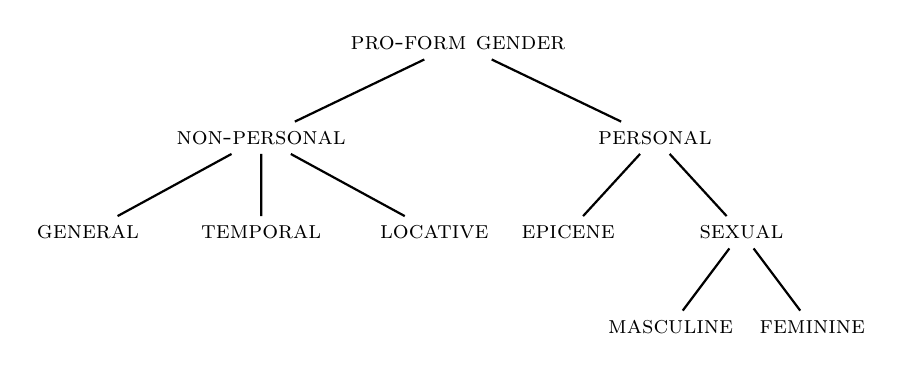
\begin{tikzpicture}[
  level distance=1.2cm,
  sibling distance=3.5cm,
  every node/.style={font=\small\scshape},
  edge from parent/.style={draw, thick},
  level 1/.style={sibling distance=5cm},
  level 2/.style={sibling distance=2.2cm},
  level 3/.style={sibling distance=1.8cm}
]
\node {pro-form gender}
  child {node {non-personal}
    child {node {general}}
    child {node {temporal}}
    child {node {locative}}
  }
  child {node {personal}
    child {node {epicene}}
    child {node {sexual}
      child {node {masculine}}
      child {node {feminine}}
    }
  };
\end{tikzpicture}
\caption{Hierarchy of gender values for English pro-forms.}
\label{fig:12:hierarchy}
\end{figure}

Each subtype inherits the properties of its parent. A word with feminine gender is necessarily sexual, which is necessarily personal. A word with locative gender is necessarily non-personal. The locative and temporal subtypes are classified under gender because they participate in the same designatum-driven licensing: \mention{where} and \mention{when} presuppose a spatial or temporal construal of their antecedent just as \mention{who} presupposes a personal construal. In form-value terms, the pro-form inventory is the form side; personhood construal is the value~-- what the form contributes when deployed. All are maintained by the same coupling mechanism: designatum-driven selection matching form to value.

Table~\ref{tab:12:inventory} shows the inventory. Rows group pro-forms by syntactic function (personal pronouns, relatives/interrogatives, demonstratives, compound determinatives); columns group them by gender value. The leftmost column lists gender-neutral pro-forms~-- items that impose no presuppositional constraint on the designatum. The remaining columns list gender-sensitive items, distinguished by the personhood constraint they encode.

\begin{table}[htbp]
\caption{The pro-form gender system of English.}
\label{tab:12:inventory}
\small
\setlength{\tabcolsep}{4pt}
\centering
\begin{tabular}{@{}p{2.2cm}p{2.0cm}p{1.5cm}p{1.5cm}p{2.5cm}p{1.0cm}p{1.0cm}@{}}
\toprule
\multicolumn{1}{c}{Gender-neutral} & \multicolumn{6}{c}{Gender-sensitive} \\
\cmidrule(l){1-1} \cmidrule(l){2-7}
& \multicolumn{3}{c}{Non-personal} & \multicolumn{3}{c}{Personal} \\
\cmidrule(lr){2-4} \cmidrule(l){5-7}
& General & Temporal & Locative & Epicene & \multicolumn{2}{c}{Sexual} \\
\cmidrule(l){2-2} \cmidrule(l){3-3} \cmidrule(l){4-4} \cmidrule(l){5-5} \cmidrule(l){6-7}
& & & & & Masc & Fem \\
\midrule
\mention{they}\textsubscript{pl} & \mention{it} & \mention{then} & \mention{there} & \mention{I}, \mention{we}\textsubscript{pron}, \mention{you}\textsubscript{pron}, \mention{they}\textsubscript{sg}, \mention{one}\textsubscript{gen} & \mention{he} & \mention{she} \\
\addlinespace
\mention{whose}\textsubscript{rel} & \mention{what}, \mention{which} & \mention{when} & \mention{where} & \mention{who}, \mention{whom}, \mention{whose}\textsubscript{int} \\
\addlinespace
\mention{this}, \mention{that}\textsuperscript{†} & & & \mention{here} & \mention{we}\textsubscript{det}, \mention{you}\textsubscript{det} \\
\addlinespace
& \mention{-thing} & & \mention{-where} & \mention{-body}, \mention{-one} \\
\bottomrule
\end{tabular}
\par\smallskip\noindent\footnotesize\textit{Note.} Subscripts: \textsubscript{pl}~=~plural; \textsubscript{sg}~=~singular; \textsubscript{gen}~=~generic; \textsubscript{rel}~=~relative; \textsubscript{int}~=~interrogative; \textsubscript{pron}~=~pronoun; \textsubscript{det}~=~determiner function (as in \mention{we linguists}, \mention{you guys}). †~In fused-head function, \mention{this} and \mention{that} show constructionally-conditioned gender: neutral in specificational \mention{be} contexts and with ellipsis; non-personal elsewhere (see §\ref{sec:12:constructional}).
\end{table}

Several entries require comment. Plural \mention{they} is gender-neutral. It can refer to persons (\mention{There are some people. They are tall}) or non-persons (\mention{There are some trees. They are tall}) without constraint. Singular \mention{they}, by contrast, is ordinarily personal: \mention{There's a person. They are tall} is straightforward, while \mention{There's a tree. They are tall} is available only under marked construals (personification, jocular animacy, or a discourse shift away from strict coreference) \autocite{bjorkman2017,konnellycowper2020}. The difference is that singular \mention{they} carries a default personal presupposition; plural \mention{they} doesn't.

Similarly, relative \mention{whose} is compatible with both personal and non-personal antecedents (\mention{the person/book whose story is well known}), while interrogative \mention{whose} typically presupposes a personal possessor (\mention{Whose coat is this?}). The split reflects how these items function: relative \mention{whose} inherits its construal from the antecedent; interrogative \mention{whose} presupposes personhood independently. Non-personal uses of interrogative \mention{whose} do occur with inalienable possession (\mention{Whose leaves are these?}, asking about a tree) or when personification is contextually available, but the default is personal.

I include first- and second-person pronouns (\mention{I}, \mention{we}, \mention{you}) to show the inventory's personhood partition. These are epicene personal: they can only refer to entities construed as persons (using \mention{I} for an inanimate object requires personification), but they don't encode sexual gender. Nothing in the analysis turns on sex marking for these items.

The table reveals a system far larger than the traditional \mention{he}/\mention{she}/\mention{it} triad. The compound determinatives~-- \mention{somebody}/\mention{something}, \mention{everyone}/\mention{everything}, \mention{anywhere}/\mention{anyone}~-- participate in the same personhood partition. The relative pro-forms \mention{where} and \mention{when} encode non-personal subtypes parallel to \mention{which}.

%--- --- --- --- --- --- --- --- --- --- --- --- --- --- --- --- ---
\section{Designatum-driven gender}
\label{sec:12:designatum}
%--- --- --- --- --- --- --- --- --- --- --- --- --- --- --- --- ---

Before examining the mechanism, a clarification. The English system tracks the \term{designatum}~-- the entity as conceptualized by the speaker~-- not the referent (the real-world correlate) or the antecedent (the linguistic controller). The \term{designatum} is what a linguistic item designates; the \term{referent} is ``some independently distinguishable entity, or set of entities, in the real world'' \autocite[399]{huddleston2002}. The \term{antecedent} is the ``constituent whose meaning dictates the meaning of a pronoun or other such expression in cases of anaphora'' \autocite[295]{huddleston2005}.

This distinction is crucial. A pro-form need not have an antecedent to participate in the gender system: interrogative \mention{who} introduces an open slot whose intended value is constrained to persons even though the utterance has neither a referent nor an antecedent. The designatum need not be a token: \mention{the typical politician isn't to be trusted} designates a type, but the gender is still personal. And the designatum can diverge from the antecedent's lexical properties.

The English system differs from antecedent-driven systems in exactly this way. In Spanish, French, or German, gender assignment is fixed on nouns and agreement spreads through NP-internal morphology. The antecedent controls the pro-form.

In English, it's the designatum~-- how the referent is conceptualized~-- that controls selection. The source provides the constraint; the pro-form satisfies it.

Consider a case of referential metonymy:

\ea[*]{\label{ex:12:metonymy}\mention{The French fries is waiting. She's upset.} \hfill \autocite{wu2025}}
\z
An NP with a default non-personal reading (\mention{the French fries}) is used to invoke a customer; subsequent anaphora tracks that metonymic designatum, yielding personal-feminine \mention{she}. The fries are, briefly, a customer with a pronoun. The antecedent's form (plural, non-personal) doesn't control the pro-form; the conceptualized source does.

Spanish is much less permissive about this kind of pro-form shift while retaining ordinary agreement with the same antecedent NP. (The English number mismatch~-- plural label, singular verb~-- reflects a menu-item construal orthogonal to the pro-form point; in Spanish I keep agreement normal to isolate the controller issue.)

\ea\label{ex:12:spanish}
    \ea[*]{\gll \mention{Las} \mention{patatas} \mention{fritas} \mention{esperan}. \mention{Él} \mention{está} \mention{enfadado}.\\
    \textsc{def.f.pl} potato.\textsc{f.pl} fried.\textsc{f.pl} wait.\textsc{3pl.pres} \textsc{3sg.m} be.\textsc{3sg.pres} angry.\textsc{m.sg}\\
    \glt Intended: `The French fries are waiting. He's upset.' [fails under intended coreference]}
    \ex[]{\gll \mention{Las} \mention{patatas} \mention{fritas} \mention{esperan}. \mention{El} \mention{señor} \mention{está} \mention{enfadado}.\\
    \textsc{def.f.pl} potato.\textsc{f.pl} fried.\textsc{f.pl} wait.\textsc{3pl.pres} \textsc{def.m.sg} gentleman.\textsc{m.sg} be.\textsc{3sg.pres} angry.\textsc{m.sg}\\
    \glt `The French fries are waiting. The gentleman is upset.'}
    \z
\z
Spanish requires grammatical agreement with the syntactic antecedent (\textit{patatas}, feminine plural), a constraint that overrides the semantic gender of the metonymic designatum. The speaker typically recasts the sentence with a human-denoting controller like \mention{\textit{el señor}} (`the gentleman') to align the syntax with the intended reference. English permits categorical shifts based on conceptualization because its gender system is maintained by the designatum directly, not by antecedent-agreement: the designatum-driven pathway is freer. This is the signature of a designatum-driven system.


%--- --- --- --- --- --- --- --- --- --- --- --- --- --- --- --- ---
\section{The inventory}
\label{sec:12:inventory}
%--- --- --- --- --- --- --- --- --- --- --- --- --- --- --- --- ---

Standard accounts keep gender within personal pronouns. \textcite[486]{huddleston2002} state that English gender is ``based purely on pronoun agreement.'' But the evidence shows the system extends across all pro-forms~-- the semantic class of items that take their meaning from another element in discourse.

What unifies pro-forms is their interpretive dependence: they have minimal
descriptive content and take their value from context~-- linguistic,
situational, or conceptual. In the clearest cases, a pronoun heads an NP
whose referent is recoverable from the discourse or situation; pro-forms like
\mention{here}/\mention{there}/\mention{then} likewise contribute a place or
time that's supplied by context rather than descriptively specified. In
interrogatives and relatives, \mention{wh}-forms don't ``stand for'' a missing
phrase so much as mark an open slot in the clause's interpretation, linked to
an answer (in questions) or to an antecedent (in relatives). This isn't a
morphosyntactic category (there's no frame that selects for ``any pro-form''),
but a semantic--pragmatic one. The gender constraint doesn't respect lexical-category
boundaries: whatever property licenses \mention{who} also licenses \mention{somebody}
and blocks \mention{something}.

The skink in the epigraph illustrates exactly this: a fleeting promotion (\mention{one's}) and immediate demotion (\mention{it}) within one sentence~-- the kind of construal shift that §\ref{sec:12:chain-coherence} will examine.

\subsection{Determinatives}
\label{sec:12:determinatives}

The compound determinatives with \mention{-body} and \mention{-one} are personal:

\ea[*]{\label{ex:12:somebody}\mention{Somebody left their coat.} \hfill [personal]}
\z
\ea[*]{\label{ex:12:somebody-bad}\mention{Somebody is in your purse.} \hfill [under construal: referring to an object]}
\z
Example (\ref{ex:12:somebody-bad}) is ungrammatical unless \mention{somebody} refers to a person who is in the purse. These are epicene~-- they don't encode sex~-- but they do encode the personal/non-personal distinction.

The compound determinatives with \mention{-thing} and \mention{-where} are non-personal:

\ea[*]{\label{ex:12:something}\mention{Something is on the table.} \hfill [non-personal]}
\z
\ea[*]{\label{ex:12:something-bad}\mention{Everything enjoyed themselves.} \hfill [under construal: personal referents]}
\z
Example (\ref{ex:12:something-bad}) requires personification to be grammatical. The boundary is discourse-driven rather than syntactically hard~-- exactly the HPC-style graded edge we expect.

\subsection{Relative pro-forms}
\label{sec:12:relative-proforms}

The distinction between \mention{where}/\mention{when} and \mention{which} parallels the distinction between \mention{who} and \mention{which}:

\ea[*]{\label{ex:12:room-where}\mention{the room where/\ungram which the painting was done} \hfill [room as location]}
\z
\ea[*]{\label{ex:12:room-which}\mention{the room which/\ungram where was painted} \hfill [room as patient]}
\z

\ea[*]{\label{ex:12:2010-when}\mention{2010, when/\ungram which I left} \hfill [as time]}
\z
\ea[*]{\label{ex:12:2010-which}\mention{2010, which/\ungram when has 365 days} \hfill [as entity]}
\z
The same source (\mention{room}, \mention{2010}) takes different pro-forms depending on how it's conceptualized. This is designatum-driven selection applied to locative and temporal subtypes.

A note on apparent avoidance. English relative clauses permit \mention{that} (a subordinator functioning as marker) and bare relatives without any overt relative word: \mention{the doctor that I saw}, \mention{the doctor I saw}. These aren't gender-neutral pro-forms~-- they're structurally different constructions that happen to sidestep the \mention{who}/\mention{which} choice. Their availability doesn't undermine the gender system; it simply means speakers can use a different construction when they would rather not take a position on the metaphysics.


%--- --- --- --- --- --- --- --- --- --- --- --- --- --- --- --- ---
\section{How the system holds together}
\label{sec:12:coupling}
%--- --- --- --- --- --- --- --- --- --- --- --- --- --- --- --- ---

\subsection{Chain coherence}
\label{sec:12:chain-coherence}

Once a designatum is construed as personal or non-personal within a reference chain, mixing is disfavoured. Consider:

\ea[*]{\label{ex:12:dog-chain-a}\mention{That's the dog \uline{who} attacked \uline{his} owner.} \hfill [personal chain]}  
\z
\ea[*]{\label{ex:12:dog-chain-b}\mention{That's the dog \uline{which} attacked \uline{its} owner.} \hfill [non-personal chain]}
\z
\ea[*]{\label{ex:12:dog-chain-c}\mention{That's the dog \uline{which} attacked \uline{his} owner.} \hfill [mixed]}
\z
\ea[*]{\label{ex:12:dog-chain-d}\mention{That's the dog \uline{who} attacked \uline{its} owner.} \hfill [mixed]}
\z
Examples (\ref{ex:12:dog-chain-a}) and (\ref{ex:12:dog-chain-b}) are fully acceptable~-- coherent personal and non-personal chains. Examples (\ref{ex:12:dog-chain-c}) and (\ref{ex:12:dog-chain-d}) are degraded~-- the chain starts in one gender and shifts to another mid-sentence.

This is \term{chain-internal coherence}. The constraint isn't absolute~-- discourse can independently reclassify a designatum (personification, stance shift)~-- but absent such cues, speakers prefer consistency within a reference chain. Attested mixed chains do occur, but they almost always involve a shift in stance. Recall the skink in the epigraph: \mention{losing \emph{one's} tail} (generic personal) followed by \mention{\emph{it} seems} (non-personal). The shift marks a move from a generic \enquote{experiencer} perspective to a biological description. Similarly, speakers discussing ships or infants may toggle between \mention{she}/\mention{he} and \mention{it} as their emotional distance varies. What's rare is a mix without a motive.

The effect is strongest in online processing: mixed chains create a local mismatch that invites repair or reinterpretation, and that repair pressure is itself a stabilizer of the coupling.

Chain coherence is a maintenance mechanism. It stabilizes the personhood assignment across discourse, reinforcing the clustering of pro-forms around a shared construal. This is the English analogue to French NP-internal concord: in French, gender coherence is enforced morphologically across determiners, adjectives, and participles; in English, it's enforced referentially across the pro-forms in a chain.

\subsection{The coupling}
\label{sec:12:coupling-subsec}

We now have the architecture (Figure~\ref{fig:12:hierarchy}). On the semantic side sits the \term{personhood cluster}: the conceptual properties that make a referent construable as a person. These cluster because personhood is a natural cognitive category, grounded in Theory of Mind and social cognition \autocite{waytz2010}.

Person-attribution, as I use it, tracks a cluster of features: potential for reciprocal interaction, nameability, attribution of intentions, membership in the speaker's circle of concern. This is folk-psychological personhood~-- the kind speakers attribute in online cognition~-- not the social-recognition sense invoked in debates about rights or legal standing. \textcite{dennett1976} lists formal conditions for personhood (rationality, consciousness, reciprocal treatment, self-awareness); I use these illustratively, not as necessary conditions that speakers compute. What matters is that these features cluster~-- Theory of Mind operates on them as a package~-- and that the clustering is cognitively basic and socially consequential.

Two kinds of personhood construal should be distinguished. In most cases, personhood is a \term{default construal}: \mention{the doctor} evokes a person without the speaker doing anything special. In others, personhood is \term{locally imposed}: \mention{Who's a good boy?} addressed to a dog requires active construal work. The maintenance story tracks both. Defaults are entrenched through ordinary usage; local impositions require discourse cues and carry interactional meaning (affection, stance, humour). The system accommodates both because the coupling is bidirectional: form can signal construal, and construal can license form.

On the lexico-grammatical side sits the \term{pro-form inventory}: the gender-sensitive lexical items and their distributional constraints: the personal pronouns (\mention{he}/\mention{she}/\mention{it}/\mention{they}), the pro-nominal \mention{one}, \mention{who}/\mention{which}, \mention{-body}/\mention{-thing} in compound determinatives, and designated slots for personal and non-personal reference. (Pro-form is a semantic grouping; what I'm tracking here is its \emph{realization}~-- the specific forms and where they're licensed.)

The two clusters are coupled by \term{designatum-driven inference}. When speakers produce a pro-form, they signal how they're construing the referent. When hearers process a pro-form, they infer the construal. Form cues construal; construal constrains form. This coupling is the category we recognize as English gender.

This parallels the bidirectional inference that couples individuation to count morphosyntax (Chapter~\ref{ch:countability}) and identifiability to deitality (Chapter~\ref{ch:definiteness-and-deitality}). The coupling is what produces the HPC signature: properties that statistically co-occur, maintained by causal mechanisms, with instability at the edges.

\subsection{The machinery of maintenance}
\label{sec:12:maintenance}

Chapter~\ref{ch:stabilizers} surveyed some of the general machinery that maintains linguistic kinds: acquisition, entrenchment, alignment, transmission. That list was explicitly incomplete; no theory of linguistic kinds can enumerate every stabilizing force. For pro-form gender, at least three domain-specific channels are visible.

\term{Cognitive grounding} explains why acquisition succeeds. As noted above (§\ref{sec:12:coupling-subsec}), the person/non-person boundary is mapped onto a pre-existing conceptual distinction that infants acquire before language begins \autocite{csibra2003,carey2009}. Because the conceptual cluster is already in place, children don't have to induce it from pro-form distributions~-- they just have to learn which forms map onto which region of an existing landscape. This is why acquisition of English pro-form gender is fast and robust. The empirical footprint: children should produce personal pro-forms for robots and animals that pass Theory-of-Mind tests, and non-personal pro-forms for entities that fail them, even before they can articulate why.

\term{Semantic transparency} explains why transmission preserves the coupling. The mapping from personhood to pro-form is largely predictable: if you know a referent is construed as a person, you can predict the pro-form inventory it will take. Compare French gender, where assignment is arbitrary and must be learned item by item, or English countability, where object-mass nouns like \mention{furniture} create opaque exceptions. English pro-form gender has fewer such mismatches: the \mention{who}/\mention{which} alternation tracks personhood with high fidelity. This transparency means the system can be reconstructed from limited input~-- what Chapter~\ref{ch:stabilizers} called \term{learnability filtering}. Children acquiring English don't produce the persistent paradigmatic gender-agreement errors characteristic of antecedent-gender languages, though direct acquisition studies of the \mention{who}/\mention{which} contrast specifically remain sparse. The empirical footprint: novel entities (AI assistants, fictional creatures) should be rapidly and consistently assigned pro-forms once their personhood status is pragmatically established, without explicit instruction.

\term{Alignment and repair} explains why the coupling is enforced in real time. Consider a constructed repair:

\begin{quote}
A: \mention{The new surgeon started today. Is he any good?}\\
B: \mention{\emph{She}. Dr. Patel's a woman.}
\end{quote}

\noindent The correction is immediate, unmarked, and socially meaningful. The point isn't that speakers consult a rulebook; it's that the mismatch is interactionally loud. Gender mismatches are charged in a way that many grammatical errors aren't: calling a person \mention{it} is an insult; misgendering someone with \mention{he} when \mention{she} is appropriate triggers conversational repair \autocite{mcconnell-ginet2014}. This repair pressure operates through what Chapter~\ref{ch:stabilizers} called \term{interactive alignment}: interlocutors converge on shared construals, and deviations are corrected. The social stakes amplify the mechanism~-- gender isn't just about communication; it's about recognition.

The pressure can also work in reverse~-- resisting innovation rather than enforcing existing norms. A younger speaker who says \mention{My partner called~-- they're running late} may prompt an older hearer to ask \mention{He or she?}, treating singular \mention{they} for a specific individual as underspecified rather than complete. The negotiation reveals competing norms rather than a shared one, and it's exactly where variation survives: alignment stabilizes whichever system the interlocutors happen to share, but when systems diverge, the repair attempt exposes the crack.

The empirical footprint: gender corrections should be faster and more frequent than corrections for other grammatical mismatches (e.g., number disagreement), and corpus data should show that gender repairs cluster in contexts where personhood or sex attribution is socially consequential.

These three channels~-- cognitive grounding, semantic transparency, alignment and repair~-- don't exhaust the mechanisms, but they illustrate how the general stabilizers from Chapter~\ref{ch:stabilizers} operate in this domain. The stability of pro-form gender emerges from their convergence: the conceptual cluster is pre-linguistic; the form-meaning mapping is reconstructible; violations are repaired in real time. Other forces~-- register conventions, prescriptive teaching, literary tradition~-- doubtless contribute; the point isn't to close the list but to show that the coupling is actively maintained.

\subsection{What the HPC framing buys}
\label{sec:12:hpc-payoff}

A sceptical reader might ask: why invoke HPC machinery at all? Why not say that each pro-form simply carries its own selectional presupposition~-- \mention{who} presupposes a personal referent, \mention{which} presupposes a non-personal one~-- and leave it there? Item-by-item presuppositions are simpler than coupled clusters.

The answer is that item-by-item presuppositions don't explain the system's behaviour. Three phenomena require more than local selectional restrictions.

First, \term{bidirectional inference}. If pro-forms merely carried presuppositions, hearers would use form to filter referent candidates~-- ruling out non-persons for \mention{who}, ruling out persons for \mention{which}. But the inference also runs the other way: hearers use \mention{who} to \emph{attribute} personal construal, even when the referent is non-human. \mention{The dog who bit me} doesn't just filter for dogs already construed as persons; it \emph{invites} that construal. This is coupling, not selection.

Second, \term{chain coherence}. If gender were just local presupposition, mixed chains (\mention{who... it}) should be as acceptable as any other presupposition shift within discourse. They aren't. The dispreference for mixed chains is a \emph{system-level} constraint~-- it tracks construal stability across the chain, not just satisfaction of local presuppositions. That's the signature of a maintained coupling, not a collection of independent filters.

Third, \term{boundary cases tracking the same dimension}. The boundary cases~-- pets, collectives, infants, robots~-- don't scatter randomly. They cluster along the personhood dimension. If each pro-form had independent presuppositional content, we would expect idiosyncratic variation: \mention{who} might extend to animals, \mention{somebody} might not. Instead, the entire inventory shifts together when personhood is uncertain. That's what coupled clusters do.

The HPC framing doesn't add complexity for its own sake. It explains why the system behaves as a system: why inference is bidirectional, why chains cohere, why boundaries track a shared dimension. Item-by-item presuppositions would predict a looser, more heterogeneous pattern~-- exactly what we don't see.

%--- --- --- --- --- --- --- --- --- --- --- --- --- --- --- --- ---
\section{Evidence and limits}
\label{sec:12:evidence}
%--- --- --- --- --- --- --- --- --- --- --- --- --- --- --- --- ---

\subsection{The maintenance spectrum}
\label{sec:12:maintenance-spectrum}

Gender systems differ not just in their inventories but in \emph{what maintains them}. The contrast between English and French illustrates the extremes; German sits between \autocite{corbett1991,audring2009}.

English pro-form gender is \term{designatum-driven}: the form tracks how the speaker construes the referent. The metonymy example in §\ref{sec:12:designatum} showed this~-- \mention{the French fries... she} is possible because the pro-form follows the conceptualized customer, not the grammatical antecedent. The system is maintained by a live semantic link: form and meaning travel together because the coupling is transparent.

French gender is \term{antecedent-driven}: the pro-form tracks the grammatical gender of the antecedent NP, regardless of the referent's properties. The same metonymy fails:

\ea[*]{\label{ex:12:french-fries}\gll \mention{Les} \mention{frites} \mention{attendent}. \mention{Il} \mention{est} \mention{en} \mention{colère}.\\
\textsc{def.f.pl} fry.\textsc{f.pl} wait.\textsc{3pl.pres} \textsc{3sg.m} be.\textsc{3sg.pres} in anger\\
\glt Intended: `The fries are waiting. He's upset.' [fails under intended coreference]}
\z

\noindent The speaker can't use masculine \mention{il} to track a male customer if the antecedent \mention{les frites} is grammatically feminine. The form-meaning link is dead: French gender is maintained by \term{pure entrenchment}~-- item-by-item memorization of arbitrary noun-class assignments, reinforced by NP-internal concord.

German is the hybrid. Nouns carry grammatical gender (\mention{der Tisch} `the table', masculine; \mention{die Lampe} `the lamp', feminine; \mention{das Mädchen} `the girl', neuter). But pronouns can override the antecedent's grammatical gender when the referent's natural gender is salient:

\ea[*]{\label{ex:12:german-girl}\gll \mention{Das} \mention{Mädchen} \mention{kam} \mention{herein}. \mention{Sie} \mention{lächelte}.\\
\textsc{def.n} girl.\textsc{n} came in. \textsc{3sg.f} smiled.\\
\glt `The girl came in. She smiled.'}
\z

\noindent The antecedent \mention{das Mädchen} is grammatically neuter, but the pronoun \mention{sie} is feminine~-- tracking the referent's natural gender, not the noun's grammatical class. German gender is maintained by \emph{two mechanisms in tension}: entrenchment of noun-class assignment, and semantic override in pronominal anaphora.

This is the \term{maintenance spectrum}. At one end, English: semantically transparent, designatum-driven, clustering held together by a live conceptual distinction. At the other end, French: semantically arbitrary, antecedent-driven, clustering held together by morphological entrenchment. French gender shows \term{mechanistic drift} (Chapter~\ref{ch:projectibility}): whatever semantic triggers may once have motivated the masculine/feminine split have long faded, but entrenchment maintains the forms. German sits between~-- two mechanisms in tension, neither fully dominant.

The HPC framework predicts different profiles. English gender should be easy to acquire (transparent mapping) but potentially unstable under pressure (no formal redundancy). French gender should be hard to acquire (arbitrary assignment) but stable once learned (reinforced by concord). German should show characteristic acquisition errors where the two systems conflict~-- and it does: children often produce natural-gender pronouns for grammatical-neuter human nouns. The ``same'' category has different ontological status depending on what maintains it.

\subsection{Cross-linguistic scope}
\label{sec:12:cross-linguistic}

Is pro-form gender an English peculiarity or a cross-linguistic pattern?

The personhood distinction appears remarkably widespread. \textcite{haspelmath1997} notes that ``the distinction between human and non-human referents is made practically everywhere (`who' vs.\ `what', `somebody' vs.\ `something'), even in languages where humanness isn't very prominent elsewhere in the grammar'' (34--35). Languages with rich antecedent-driven gender (Spanish \mention{quién}/\mention{qué}, German \mention{wer}/\mention{was}, French \mention{qui}/\mention{quoi}) still make the personhood split in their interrogative and indefinite systems \autocite{corbett1991,dahl2000}. First- and second-person pronouns are epicene in many languages that otherwise mark sex in the third person, suggesting that the personhood axis~-- distinguishing speech-act participants from non-participants~-- is cross-linguistically more stable than sex-based contrasts. The personhood partition may be cognitively more basic than the particular morphosyntactic systems that realize it.

What's distinctive about English isn't the personhood distinction itself but its \term{scope}. Because English lacks NP-internal gender agreement, the designatum-driven pathway is unconstrained by formal concord. Speakers can shift a referent's construal without generating agreement violations. The \mention{who}/\mention{which} alternation, the \mention{-body}/\mention{-thing} compounds, and the chain-coherence effects are all more prominent in English precisely because they're not overridden by noun-class agreement.

Dialectal variation within English shows the system's parameters. \textcite{siemund2008} documents varieties (Southwest England, Newfoundland, Tasmania) where the personal/non-personal cut shifts: \mention{he} and \mention{she} extend to inanimates based on a mass/count distinction rather than personhood. The hierarchy's structure remains stable; its semantic basis varies. This suggests the architecture is robust but its semantic grounding is a parameter that communities can tune.

\subsection{Passing the tests}
\label{sec:12:tests}

Chapter~\ref{ch:failure-modes} introduced the Two-Diagnostic Test for genuine HPC kinds: high projectibility and robust homeostasis.

Knowing a pro-form's gender predicts its distribution. If you know \mention{somebody} is personal, you can predict it will combine with personal predicates, take personal reflexives (\mention{themselves}), and resist non-personal contexts. If you know \mention{which} is non-personal, you can predict it can't take human antecedents without personification.

Crucially, knowing the designatum's construal predicts pro-form selection. If you know the speaker is construing a pet as personal, you can predict \mention{who} over \mention{which}, \mention{he}/\mention{she} over \mention{it}. The predictions are bidirectional: from form to construal, from construal to form.

The clustering is maintained by mechanisms. Acquisition transmits the system as a unit; entrenchment preserves high-frequency patterns; alignment provides real-time stabilization; transmission filters for learnability. Perturb any mechanism~-- expose children to non-standard input, isolate speakers from conversational feedback~-- and the cluster should degrade. But it won't scatter randomly; the degradation will track the mechanisms involved.

The clustering isn't just a statistical regularity. It's causally maintained.

\subsection{Where the clusters slip}
\label{sec:12:slippage}

By ``slippage'' I mean cases where the two clusters that normally travel together~-- personhood construal and the pro-form inventory that encodes it~-- are pulled apart by independent pressures. The result isn't random noise: the same boundary cases recur, and the same repairs and preferences reassert the coupling. The interest of these cases is diagnostic: they show which mechanisms are doing the stabilizing, and where other systems~-- number, specificity, register~-- interfere with the personhood signal.

\subsubsection{Boundary designata}
\label{sec:12:boundary}

Some referents sit at the boundary of personhood attribution. Pets are the paradigm case. \textcite{shirvertesh2012} demonstrates that pet-keeping licenses flexible personhood construal: the same animal can be a person in one context and not in another. This flexibility surfaces in pro-form choice:

\ea[*]{\label{ex:12:cat-it}\mention{The cat licked its paw.} \hfill [non-personal default]}
\z
\ea[*]{\label{ex:12:cat-she}\mention{Poor Whiskers! She's not feeling well.} \hfill [personal]}
\z
Same referent, different construals~-- and different pro-forms. The variability here isn't a partial breakdown of the coupling; it's the \emph{expected} outcome when the semantic cluster itself is gradient. Because personhood is genuinely uncertain for these referents, the system permits controlled alternation. What stabilizes the pattern is chain coherence: having chosen personal or non-personal for a given referent in a given discourse, speakers prefer to stay consistent.

\subsubsection{Interference from number}
\label{sec:12:number}

Collective nouns present a case where another grammatical cluster~-- number and mereology~-- interferes with the personhood signal:

\ea[*]{\label{ex:12:team-its}\mention{The team has scored its first goal.} \hfill [singular, non-personal]}
\z
\ea[*]{\label{ex:12:team-their}\mention{The team have scored their first goal.} \hfill [plural, personal]}
\z
The variation tracks construal: team-as-entity versus team-as-members. But this is primarily notional versus grammatical number, not gender per se. The personhood of the individual members isn't in doubt; what varies is whether they're accessed as individuals or aggregated into a single non-personal entity.

Dialect and register norms amplify the variation. British English more readily accepts plural verb agreement with singular collective heads; American English more strongly prefers singular \autocite{bock2006}. What's interesting for the HPC analysis is that the combination of singular verb with plural personal anaphora (\mention{The team has changed their strategy}) is widely tolerated~-- the two agreement systems (verbal, pronominal) can diverge when pulled by different pressures. The mechanism that stabilizes the pattern is standardization pressure: edited prose tends to favour singular--singular or plural--plural; informal speech permits the mix.

A related case is \mention{much}, which is strictly non-personal: \mention{*Much arrived late} is ungrammatical with intended personal reference. But this may not be a gender constraint per se. Persons are typically individuated~-- conceptualized as countable entities~-- and \mention{much} quantifies over mass. The incompatibility may follow from count/mass semantics rather than from an independent personhood presupposition on \mention{much}. If so, the non-personal status of \mention{much} is an epiphenomenon of the count/mass system, not a direct participant in the gender coupling. This is a case where two maintenance mechanisms~-- individuation and personhood~-- happen to align, making it hard to say which is doing the work.

\subsubsection{Competition from other pressures}
\label{sec:12:competition}

Human infants, paradigmatic persons, can take non-personal \mention{it}:

\ea[*]{\label{ex:12:baby-it}\mention{The baby was crying because it was hungry.}}
\z
This isn't a denial of personhood. It reflects competition between personhood and other communicative pressures~-- particularly sex-marking and specificity. When the infant's sex is unknown or irrelevant, \mention{it} can avoid the sex-based \mention{he}/\mention{she} alternation. In generic construals (\mention{A baby needs its mother}), the kind-level reading aligns naturally with non-personal anaphora. And in some contexts, as \textcite{mcconnell-ginet2014} notes, the choice of \mention{it} can carry ideological weight~-- positioning the infant as not-yet-fully-a-person, though this isn't the default reading.

The slippage here is diagnostic: it shows that the personhood--pro-form coupling can be loosened when other communicative goals take priority. What stabilizes the pattern is semantic transparency: when a speaker does construe an infant as personal, the system snaps back to \mention{he}/\mention{she}/\mention{they}. As singular \mention{they} spreads as a sex-neutral personal pronoun, \mention{it} for infants may wane~-- replaced by a form that's unambiguously personal without requiring sex specification.

\subsubsection{Lexeme-specific anchoring}
\label{sec:12:anchoring}

Not all non-personal pro-forms behave identically when chains continue. Relative \mention{which}, tethered to an antecedent NP, appears more permissive for some speakers in allowing later personal anaphora, even though the resulting mixed chain is typically marked:

\ea[*]{\label{ex:12:which-chain}\mention{The dog which attacked the woman ran away. The police never caught him.} \hfill [upgrade within chain]}
\z
The antecedent (\mention{the dog}) supplies enough information~-- animacy, individuality~-- that hearers can reconstruct a personal designatum and accommodate the shift.

But \mention{what} in free relatives and \mention{something} are systematically underspecified. They lack a full NP antecedent to inherit features from, so there's less material for hearers to anchor a promoted personal construal:

\ea[*]{\label{ex:12:what-chain}\mention{What attacked the woman ran away. The police never caught him.}}
\z
\ea[*]{\label{ex:12:something-chain}\mention{Something attacked the woman. The police never caught him.} \hfill [with coreference]}
\z
The contrast, if these judgments hold up, isn't simple gradience within the non-personal domain; it's a difference in discourse anchoring and feature support. Relative \mention{which} points to an existing NP whose descriptive content can sometimes license an \enquote{upgrade}; \mention{what} and \mention{something} provide no comparable antecedent to inherit from, so the chain more strongly resists promotion to personal. The mechanism that stabilizes the pattern is chain coherence: when the anchor is weak, shift is blocked or sharply degraded.

\subsubsection{Constructional interference: the demonstratives}
\label{sec:12:constructional}

The demonstratives \mention{this} and \mention{that} present a different kind of slippage~-- one driven not by properties of the designatum but by the syntactic construction in which the pro-form appears.

In fused determiner-head function, demonstratives aren't simply gender-neutral. Their gender is \term{constructionally conditioned}:

\ea[*]{\label{ex:12:demo-pers-blocked}\mention{She chatted with that.} \hfill [personal blocked]}
\z
\ea[*]{\label{ex:12:demo-spec}\mention{This is Yoko.} / \mention{This is an acorn.} \hfill [specificational \mention{be}: neutral]}
\z
\ea[*]{\label{ex:12:demo-ellipsis}\mention{She chatted with this person and that.} \hfill [ellipsis: personal OK]}
\z

Example (\ref{ex:12:demo-pers-blocked}) shows that personal reference is blocked in bare fused-head contexts~-- unless the speaker intends depersonalization as an insult. But examples (\ref{ex:12:demo-spec}) and (\ref{ex:12:demo-ellipsis}) show that personal reference is licensed in two environments: specificational \mention{be} constructions and ellipsis with a recoverable head noun.

The pattern isn't random. Specificational \mention{be} and ellipsis both provide structural support that bare fused-heads lack. In \mention{This is Yoko}, the post-copular complement supplies the personhood information; the demonstrative merely points. In \mention{She chatted with this person and that}, the elided head \mention{person} is recoverable from the first conjunct. Without such support, the demonstrative defaults to non-personal, and personal construal is unavailable.

This is constructional interference with the gender coupling. The same lexeme~-- \mention{that} as a fused head~-- behaves as non-personal in one syntactic frame and as gender-neutral in another. The stabilizing mechanism is \term{constructional support}: certain syntactic environments carry licensing conditions that override the default constraint. This parallels the lexeme-specific anchoring discussed above: relative \mention{which} with a full NP antecedent can license chain upgrades that underspecified \mention{what} can't. Here, the specificational \mention{be} construction and ellipsis structures provide the anchoring that bare demonstratives lack.

The demonstratives, then, sit uneasily in the gender-neutral column of Table~\ref{tab:12:inventory}. In fused-head function, they're neutral only when the construction provides enough structure to license personal reference; otherwise, they default to non-personal. This constructional sensitivity is exactly the kind of graded, context-dependent behaviour that HPC kinds predict~-- and it shows how grammatical structure can modulate the personhood--pro-form coupling.


%--- --- --- --- --- --- --- --- --- --- --- --- --- --- --- --- ---
\section{Looking forward}
\label{sec:12:transition}
%--- --- --- --- --- --- --- --- --- --- --- --- --- --- --- --- ---

Pro-form gender is a localized system. The relevant constraints are carried by a specific semantic class of lexical items~-- those that function as pro-forms~-- and enforced across anaphoric chains. The coupling between personhood and morphosyntax is tight within that domain: the category is real because it's maintained, and maintained because it's real. Lexical-gender systems like French exhibit \term{mechanistic drift} in the other direction: the semantic triggers have faded, but entrenchment maintains the forms (Chapter~\ref{ch:projectibility}).

The final case study pushes to the widest scope. Lexical categories like \term{noun} and \term{verb} look strikingly stable cross-linguistically, while \term{adjective} and \term{adposition} vary dramatically. If these are HPC kinds, the mechanisms that maintain them must be far more diffuse~-- operating across the entire grammar, not just within a circumscribed inventory. Chapter~\ref{ch:lexical-categories} asks what happens when the coupling is weak, the mechanisms are partial, and the cluster boundaries are contested.
